%!TEX TS-program = xelatex
\documentclass[12pt, a4paper, oneside]{article}

% Можно вставить разную преамбулу
% пакеты для математики
\usepackage{amsmath,amsfonts,amssymb,amsthm,mathtools}  
\mathtoolsset{showonlyrefs=true}  % Показывать номера только у тех формул, на которые есть \eqref{} в тексте.

\usepackage[british,russian]{babel} % выбор языка для документа
\usepackage[utf8]{inputenc}          % utf8 кодировка

% Основные шрифты 
\usepackage{fontspec}         
\setmainfont{Linux Libertine O}  % задаёт основной шрифт документа

% Математические шрифты 
\usepackage{unicode-math}     
\setmathfont[math-style=upright]{euler.otf} 

\setmathfont[range={\mathbb, \mathop, \heartsuit, \angle, \smile, \varheartsuit}]{Asana-Math.otf}

%%%%%%%%%% Работа с картинками и таблицами %%%%%%%%%%
\usepackage{graphicx} % Для вставки рисунков                
\usepackage{graphics}
\graphicspath{{images/}{pictures/}}   % папки с картинками

\usepackage[figurename=Картинка]{caption}

\usepackage{wrapfig}    % обтекание рисунков и таблиц текстом

\usepackage{booktabs}   % таблицы как в годных книгах
\usepackage{tabularx}   % новые типы колонок
\usepackage{tabulary}   % и ещё новые типы колонок
\usepackage{float}      % возможность позиционировать объекты в нужном месте
\renewcommand{\arraystretch}{1.2}  % больше расстояние между строками


%%%%%%%%%% Графики и рисование %%%%%%%%%%
\usepackage{tikz, pgfplots}  % языки для графики
%\pgfplotsset{compat=1.16}

\usepackage{todonotes} % для вставки в документ заметок о том, что осталось сделать
% \todo{Здесь надо коэффициенты исправить}
% \missingfigure{Здесь будет Последний день Помпеи}
% \listoftodos --- печатает все поставленные \todo'шки

\usepackage{multicol}

%%%%%%%%%% Внешний вид страницы %%%%%%%%%%

\usepackage[paper=a4paper, top=20mm, bottom=15mm,left=20mm,right=15mm]{geometry}
\usepackage{indentfirst}    % установка отступа в первом абзаце главы

\usepackage{setspace}
\setstretch{1.15}  % межстрочный интервал
\setlength{\parskip}{4mm}   % Расстояние между абзацами
% Разные длины в LaTeX: https://en.wikibooks.org/wiki/LaTeX/Lengths

% свешиваем пунктуацию
% теперь знаки пунктуации могут вылезать за правую границу текста, при этом текст выглядит ровнее
\usepackage{microtype}

% \flushbottom                            % Эта команда заставляет LaTeX чуть растягивать строки, чтобы получить идеально прямоугольную страницу
\righthyphenmin=2                       % Разрешение переноса двух и более символов
\widowpenalty=300                     % Небольшое наказание за вдовствующую строку (одна строка абзаца на этой странице, остальное --- на следующей)
\clubpenalty=3000                     % Приличное наказание за сиротствующую строку (омерзительно висящая одинокая строка в начале страницы)
\tolerance=10000     % Ещё какое-то наказание.

% мои цвета https://www.artlebedev.ru/colors/
\definecolor{titleblue}{rgb}{0.2,0.4,0.6} 
\definecolor{blue}{rgb}{0.2,0.4,0.6} 
%\definecolor{red}{rgb}{1,0,0.2} 
\definecolor{green}{rgb}{0, 0.6, 0}
\definecolor{purp}{rgb}{0.4,0,0.8} 

\definecolor{red}{RGB}{213,94,0}
\definecolor{yellow}{RGB}{240,228,66}


% цвета из geogebra 
\definecolor{litebrown}{rgb}{0.6,0.2,0}
\definecolor{darkbrown}{rgb}{0.75,0.75,0.75}

% Гиперссылки
\usepackage{xcolor}   % разные цвета

\usepackage{hyperref}
\hypersetup{
	unicode=true,           % позволяет использовать юникодные символы
	colorlinks=true,       	% true - цветные ссылки
	urlcolor=blue,          % цвет ссылки на url
	linkcolor=black,          % внутренние ссылки
	citecolor=green,        % на библиографию
	breaklinks              % если ссылка не умещается в одну строку, разбивать её на две части?
}

% меняю оформление секций 
\usepackage{titlesec}
\usepackage{sectsty}

% меняю цвет на синий
\sectionfont{\color{titleblue}}
\subsectionfont{\color{titleblue}}

% кружочки у цифр в секциях
\renewcommand{\thesection}{\arabic{section}}

% https://ru.overleaf.com/learn/latex/Sections_and_chapters

% выбрасываю нумерацию страниц и колонтитулы 
%\pagestyle{empty}

% синие круглые бульпоинты в списках itemize 
\usepackage{enumitem}

\definecolor{itemizeblue}{rgb}{0, 0.45, 0.70}

\newcommand*{\MyPoint}{\tikz \draw [baseline, fill=itemizeblue, draw=blue] circle (2.5pt);}
\renewcommand{\labelitemi}{\MyPoint}

\AddEnumerateCounter{\asbuk}{\@asbuk}{\cyrm}
\renewcommand{\theenumi}{\asbuk{enumi}}

% расстояние в списках
\setlist[itemize]{parsep=0.4em,itemsep=0em,topsep=0ex}
\setlist[enumerate]{parsep=0.4em,itemsep=0em,topsep=0ex}

% эпиграфы
\usepackage{epigraph}
\setlength\epigraphwidth{.6\textwidth}
\setlength\epigraphrule{0pt}

%%%%%%%%%% Свои команды %%%%%%%%%%

% Математические операторы первой необходимости:
\DeclareMathOperator{\sgn}{sign}
\DeclareMathOperator*{\argmin}{arg\,min}
\DeclareMathOperator*{\argmax}{arg\,max}
\DeclareMathOperator{\Cov}{Cov}
\DeclareMathOperator{\Var}{Var}
\DeclareMathOperator{\Corr}{Corr}

\DeclareMathOperator{\Pois}{Pois}
\DeclareMathOperator{\Geom}{Geom}
\DeclareMathOperator{\Exp}{Exp}

%\DeclareMathOperator{\E}{\mathbb{E}}
\DeclareMathOperator{\Med}{Med}
\DeclareMathOperator{\Mod}{Mod}
\DeclareMathOperator*{\plim}{plim}

% команды пореже
\newcommand{\const}{\mathrm{const}}  % const прямым начертанием
\newcommand{\iid}{\sim i\,i\,d\,\,}  % ну вы поняли...
\newcommand{\fr}[2]{\ensuremath{^{#1}/_{#2}}}   % особая дробь
\newcommand{\ind}[1]{\mathbbm{1}_{\{#1\}}} % Индикатор события
\newcommand{\dx}[1]{\,\mathrm{d}#1} % для интеграла: маленький отступ и прямая d

% одеваем шапки на частые штуки
\def \hb{\hat{\beta}}
\def \hs{\hat{s}}
\def \hy{\hat{y}}
\def \hY{\hat{Y}}
\def \he{\hat{\varepsilon}}
\def \hVar{\widehat{\Var}}
\def \hCorr{\widehat{\Corr}}
\def \hCov{\widehat{\Cov}}

% Греческие буквы
\def \a{\alpha}
\def \b{\beta}
\def \t{\tau}
\def \dt{\delta}
\def \e{\varepsilon}
\def \ga{\gamma}
\def \kp{\varkappa}
\def \la{\lambda}
\def \sg{\sigma}
\def \tt{\theta}
\def \Dt{\Delta}
\def \La{\Lambda}
\def \Sg{\Sigma}
\def \Tt{\Theta}
\def \Om{\Omega}
\def \om{\omega}

% Готика
\def \mA{\mathcal{A}}
\def \mB{\mathcal{B}}
\def \mC{\mathcal{C}}
\def \mE{\mathcal{E}}
\def \mF{\mathcal{F}}
\def \mH{\mathcal{H}}
\def \mL{\mathcal{L}}
\def \mN{\mathcal{N}}
\def \mU{\mathcal{U}}
\def \mV{\mathcal{V}}
\def \mW{\mathcal{W}}

% Жирные буквы
\def \mbb{\mathbb}
\def \RR{\mbb R}
\def \NN{\mbb N}
\def \ZZ{\mbb Z}
\def \PP{\mbb{P}}
\def \E{\mbb{E}}
\def \QQ{\mbb Q}

\def\F{\ensuremath{\mathcal{F}}} % аналогично!

%%%%%%%%%% Теоремы %%%%%%%%%%
\theoremstyle{plain} % Это стиль по умолчанию.  Есть другие стили.
\newtheorem{theorem}{Теорема}[section]
\newtheorem{proposition}{Утверждение}[section]
\newtheorem{result}{Следствие}[section]

% убирает курсив и что-то еще наверное делает ;)
\theoremstyle{definition}         
\newtheorem*{definition}{Определение}  % нумерация не идёт вообще


%%%%%%%%%% Задачки и решения %%%%%%%%%%
\usepackage{etoolbox}    % логические операторы для своих макросов
\usepackage{environ}
\newtoggle{lecture}

\newcounter{probNum}[section]  % счётчик для упражнений 
\NewEnviron{problem}[1]{%
    \refstepcounter{probNum}% увеличели номер на 1 
    {\noindent \textbf{\large \color{titleblue} Упражнение~\theprobNum~#1}  \\ \\ \BODY}
    {}%
  }

% Окружение, чтобы можно было убирать решения из pdf
\NewEnviron{sol}{%
  \iftoggle{lecture}
    {\noindent \textbf{\large Решение:} \\ \\ \BODY}
    {}%
  }
 
% выделение по тексту важных вещей
\newcommand{\indef}[1]{\textbf{ \color{green} #1}} 

% разные дополнения для картинок
\usetikzlibrary{arrows.meta}
\usepackage{varwidth}

\usepackage[normalem]{ulem}  % для зачекивания текста

% Если переключить в false, все solution исчезнут из pdf
\toggletrue{lecture}
%\togglefalse{lecture}



\title{
\begin{center} 
\includegraphics[width=0.99\textwidth]{logo.png}
\end{center}

Посиделка 7: ЦПТ и ЗБЧ}
\date{ } %\today}

\author{Ульянкин Ппилиф}

\begin{document} % Конец преамбулы, начало файла

\maketitle

\epigraph{Много не мало.}{\textit{(Мой друг Игорь при покупке водки  в баню \newline в расчёте литр на человека)}}

В этой посиделке мы подробно поговорим о теоремах, на которых всё стоит. О законе больших чисел, ЗБЧ и центральной предельной теореме, ЦПТ. В прошлой посиделке было слишком много математики и слишком мало офигительных историй. В этой мы попробуем исправить возникший дисбаланс.


\section{Закон больших чисел в картинках}

\indef{Закон больших чисел, ЗБЧ} --- это теорема, которая говорит о том, что среднее арифметическое большого числа похожих случайных величин  «стабилизируется» с ростом их числа. 

Чтобы понять эту мысль, давайте рассмотрим простой пример. Пусть у нас в руках есть игральный кубик. Пусть $X_i$ --- число очков, которое на нём выпало при подбрасывании. Каждая сторона кубика выпадает с вероятностью $\frac{1}{6}.$ Получается, что $\E(X_i) = 3.5.$ 

Давайте будем подкидывать кубик и считать $\bar X$ по мере увеличения количества бросков. По оси $x$ отложим число бросков, по оси $y$ среднее, посчитанное по текущей выборке. По мере увеличения числа бросков, среднее значение всех выпавших исходов будет постепенно приближаться к $3.5$. Среднее арифметическое большого числа похожих случайных величин  «стабилизируется» с ростом их числа.

\begin{center} 
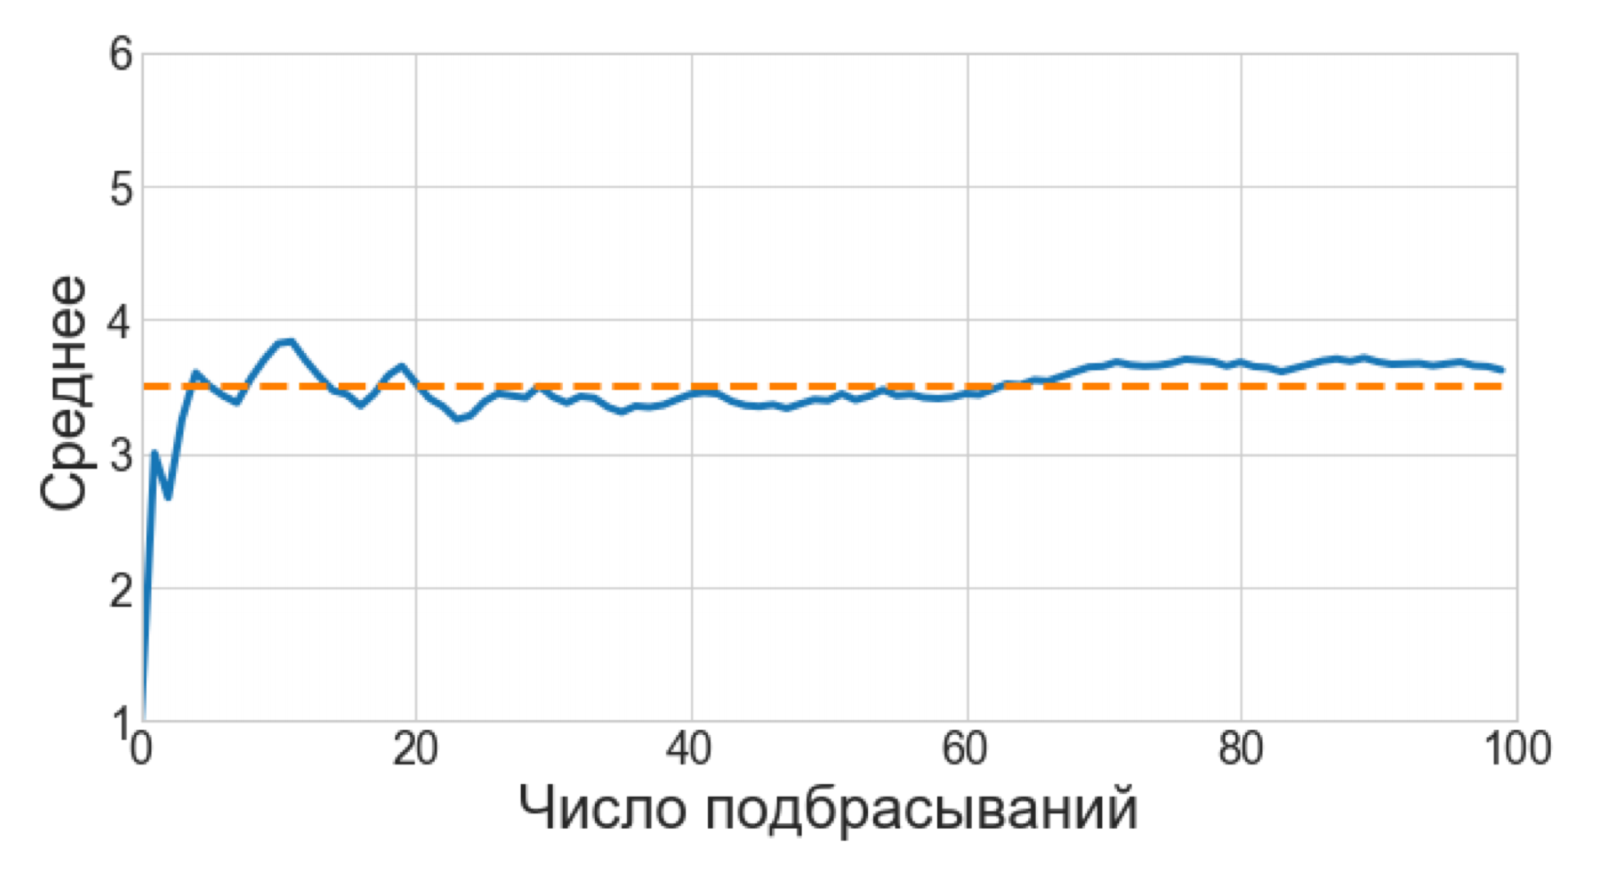
\includegraphics[width=0.8\linewidth]{lln_cube.png}
\end{center} 


\begin{theorem}{\textbf{Закон Больших Чисел (Пафнутий Львович Чебышёв)}}

Пусть $X_1, \ldots, X_n$ попарно независимые и одинаково распределённые случайные величины с конечным вторым моментом, $0 < E(X_i^2) < \infty$, тогда

$$
\bar{X}_{n} = \frac{X_1 + \ldots + X_n}{n} \stackrel{p}{\longrightarrow} E(X_1).
$$
\end{theorem}

Закон больших чисел --- офигенная теорема. Если пытаться упростить её до совсем банального высказывания, то я бы сформулировал ЗБЧ так: «Если у тебя есть страховая фирма, то ты можешь заработать бабла.» Впервые ЗБЧ разрешил зарабатывать страховым компаниям деньги в $XVI$ веке.

Люди впервые начали составлять актуарные таблицы. Это такие таблицы, где указана ожидаемая продолжительность жизни для данного возраста и пола. Люди начали собирать данные о смертности и оценивать вероятность дожития человека до определённого возраста. На этом строились тарифы на страхование. Появление подобных таблиц обязано зарождению в течение 1600-х годов теории вероятности, которая впервые объяснила людям как случайные вещи при достаточно больших масштабах сглаживаются и становятся очень даже предсказуемыми~\cite{zhlobolite}. Забавно, что изначально теорию вероятности развивали аристократы, которых заинтересовало то, как работают азартные игры\footnote{Иван, который вкладывается в крипту на всю котлету не дурак, а потенциальный отец-основатель совершенно новой ветви математики.}.

В Лондоне $2$ сентября $1666$ года случился пожар. Город горел несколько дней. Когда пожар удалось потушить, один из жителей столицы, Николас Барбон, в прошлом врач, переквалифицировался в застройщика и начал продавать страховки от пожаров. Свою фирму он назвал «Феникс». 

\begin{problem}{(Простая страховка)}
Вероятность того, что на машину во дворе упадёт дерево составляет $0.01$. Страховка в фирме Николаса стоит $10$ рублей в год. В случае, если дерево упало на машину, Николас выплачивает клиенту $2000$ рублей. Какой будет средняя прибыль его компании с одной страховки? 
\end{problem}

\begin{sol}
Пусть случайная величина $X_i$ --- прибыль с одного человека, а $\bar X$ --- средняя прибыль компании. Выпишем распределение $X_i$

\begin{center}
    \begin{tabular}{c|c|c}
    $X_i$          & $10$  & $-1990$ \\ \hline 
    $\PP(X_i = k)$ & $0.99$ & $0.01$ 
    \end{tabular}
\end{center}

По ЗБЧ 

$$
\bar X = \frac{X_1 + \ldots + X_n}{n} \stackrel{p}{\longrightarrow} E(X_i) = 10 \cdot 0.99 - 1990 ⋅ 0.01 = −10.
$$

Получается, что бизнес у Николаса убыточный. 
\end{sol}

Обратите внимание, что мы рассуждаем в предпосылке, что все случайные величины похожи друг на друга. У нас нет выбросов. В жизни они периодически происходят. С лёгкой руки Нассима Талеба такие выбросы, которые всё портят называют \indef{чёрными лебедями.} 

До $1697$ года человечество думало, что лебеди бывают только белыми. Однако голландская экспедиция обнаружила в Западной Австралии популяцию чёрных лебедей. Выражение «чёрный лебедь» используется как метафора того, что весь эмпирический опыт, который был накоплен людьми, может в один момент обесцениться из-за редкого события. Например, тот же Лондонский пожар $1666$ года --- это чёрный лебедь. Огромное количество страховых компаний разорилось из-за подобных больших катастроф. 

Секундочку... Но тогда же это означает, что ЗБЧ не применим к реальной жизни и всё, что я написал в этой главе --- это булщит. На самом деле нет. Когда мы находимся среднестатистическом мире, \indef{в Средиземье,} ЗБЧ и ЦПТ хорошо работают. Как только мы попадаем в мир хвостов распределения, \indef{в Крайнеземье,} начинаются проблемы. Но об этом более подробно мы будем говорить ниже. 

Контрольный вопрос на понимание ЗБЧ. Попробуйте ответить на него сами, а после уже смотрите сноску с верным рассуждением. Пусть мальчики и девочки рождаются равновероятно. В городе есть две больницы: большая и маленькая. В обеих принимают роды. Выяснилось, что в одной из них оценка вероятности появления мальчика составила $0.7$. В какой больнице это скорее всего произошло и почему\footnote{Скорее всего это произошло в маленькой больнице. При малых объёмах выборки вероятность отклониться от $0.5$ больше. Именно об этом говорит нам ЗБЧ.}?


\section{Центральная предельная теорема}

\indef{Центральная предельная теорема, ЦПТ,} говорит, что сумма довольно большого числа случайных величин имеет в пределе распределение близкое к нормальному, если среди этих случайных величин нет каких-то выбросов, аномалий, и они в целом друг на друга очень сильно похожи.

Снова давайте посмотрим на игральные кубики. Когда подкидываем одну игральную кость, она равновероятно может принять значение $1, 2, 3, 4, 5, 6$. Если мы подкинем игральную кость два раза, то сумма уже будет принимать значение с разными вероятностями.  Значение $2$ эта сумма примет с более низкой вероятностью, чем значение $6$. Двойку можно получить только как сумму из двух единичек, а шестёрку можно получить кучей способов. Как два и четыре, три и три, один и пять.  При этом значение $12$ тоже можно получить только одним способом. Распределение суммы будет выглядеть как треугольник. 

\begin{center} 
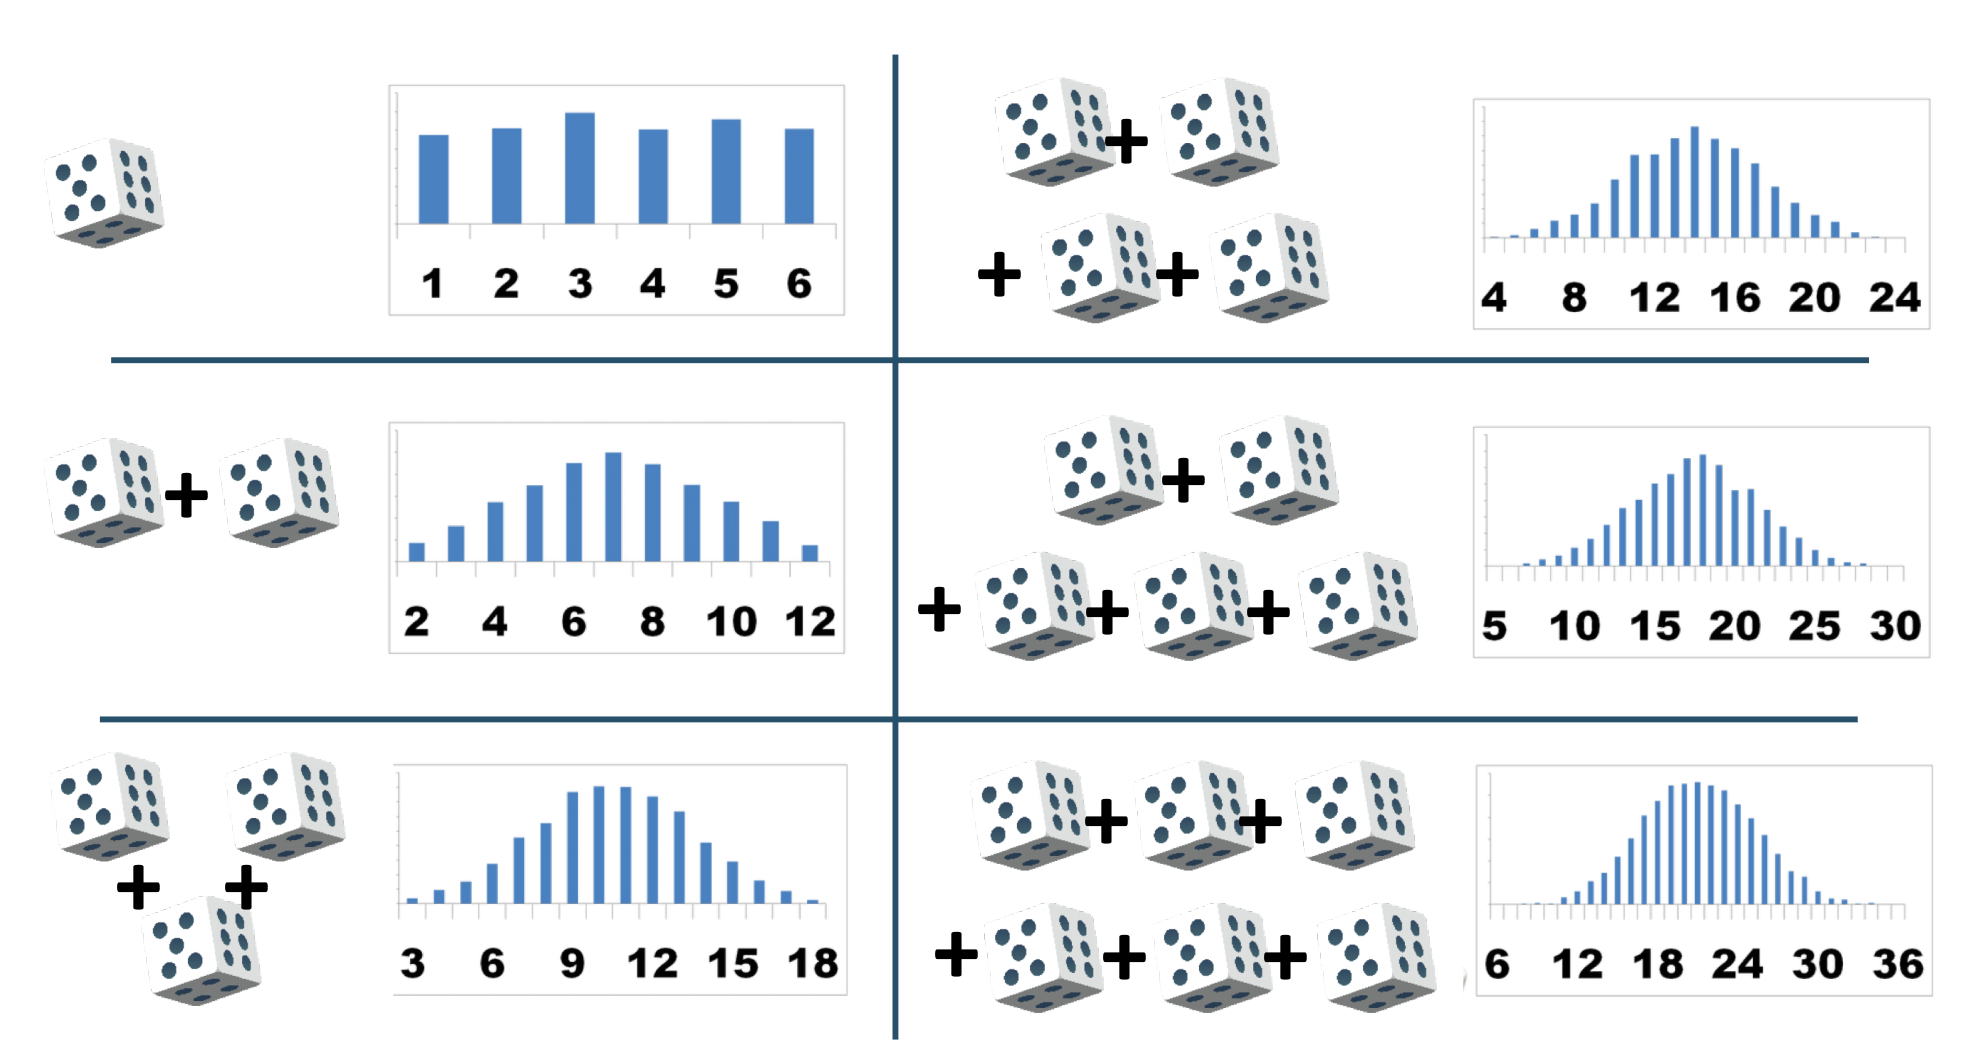
\includegraphics[width=0.95\linewidth]{clt_cube.png}
\end{center} 

Если мы подкинем $3$ игральные кости, то распределение станет еще более куполообразным, если подкинем $4$, распределение станет еще куполообразнее. Чем больше случайных величин мы будем суммировать, тем ближе к нормальному будет итоговое распределение. Именно об этом и говорит нам ЦПТ. На практике мы часто считаем средние. Именно в этом месте ЦПТ оказывается для нас хорошим помощником, на базе которого можно сделать вывод о том, насколько разнообразные значения это среднее может принимать. 

\begin{theorem}{\textbf{Центральная Предельная Теорема (Прокопий Петрович Ляпунов)}}

Пусть $X_1, \ldots, X_n$ попарно независимые и одинаково распределённые случайные величины с конечным вторым моментом, $E(X_i^2) < \infty$, тогда при $n \to \infty$ имеет место сходимость по распределению: 

$$
\bar{X} \overset{d}{\to} N \left(\E(X_i), \frac{\Var(X_i)}{n} \right)
$$

Этот же факт можно переписать немного иначе:

\[\sqrt{n} \cdot [\bar X - \E(X_i)]  \overset{d}{\to} N \left(0, \Var(X_i)\right)\]

или даже как

\[\sqrt{n} \cdot \frac{\bar{X} - \E(X_i)}{\sqrt{\Var(X_i)}}  \overset{d}{\to} N \left(0, 1\right).\]

\end{theorem}

Если говорить простым языком, то при определённых условиях сумма достаточно большого числа случайных величин имеет распределение близкое к нормальному. Есть очень большое количество формулировок ЦПТ с разными условиями и скоростями сходимости. \indef{Глобально в этих условиях главное, чтобы случайные величины были похожи и не было такого, что одна резко выделяется на фоне остальных.} 

Посмотрим еще на один пример. Предположим, что случайная величина $X$ --- время прихода Ратибора на первую пару. Если Ратибор опоздал на пару, то $X$ принимает значение того времени, на какое он опоздал. Если он пришел заранее, то случайная величина $X$ принимает отрицательное значение. Это время складывается из большого количества разных мелких случайностей. 

Сегодня утром на Ратибора прыгнул его кот, Батый. Из-за этого пришлось встать пораньше. У нас появилась случайная величина $X_1,$ которая войдёт в нашу итоговую случайную величину $X.$ Дальше Ратибор решил поесть хлопушки с тёплым молоком, но оно убежало. Пришлось убираться. Возникла задержка на $X_2.$  Дальше, автобус приехал пораньше, Ратибору повезло, но, к сожалению, по ходу своего маршрута он встал в гигантскую пробку, и из-за этого задержался ещё сильнее. 

В итоге время прихода Ратибора на пару складывается из огромного количества случайностей, которые состыкуются между собой. И если ни одна из этих случайностей не выделяется резко на фоне всех остальных, то время прихода, $X$ хорошо аппроксимируется нормальным распределением. 

Если кот часто прыгает на Ратибора очень-очень рано, и Ратибор едет на пару, не засыпая по второму кругу, нормальность сломается. Хвост, в котором Ратибор приходит заранее, будет более толстым, так как из-за кота это будет происходить намного чаще.


\begin{problem}{(Резервы для страховки)}
Портфель страховой компании состоит из $1000$ договоров, заключенных $1$
января и действующих в течение года. При наступлении страхового случая по каждому из договоров компания обязуется выплатить $1500$ рублей.

Вероятность наступления страхового события по каждому из договоров предполагается равной $0.05$ и не зависящей от наступления страховых событий по другим контрактам. Каков должен быть совокупный размер резерва страховой компании для того, чтобы с вероятностью $0.95$ она могла бы удовлетворить требования, возникающие по указанным договорам?
\end{problem}

\begin{sol}
Пусть случайная величина $X_i$ принимает значение $1$, если для $i-$го клиента наступил страховой случай. Тогда общее число страховых случаев 

\[
Y = \sum_{i=1}^n X_i \sim Bin(n=1000, p=0.05).
\]

Пусть $S$ --- размет резерва. Тогда условие на него можно записать в виде $\PP(1500 Y \leq S) = 0.95$. Решать это уравнение, используя биномиальное распределение, довольно сложно. Учитывая, что у нас много клиентов и возникновение страховых случаев распределено одинаково, мы можем воспользоваться ЦПТ

\[
\frac{1}{n} \sum_{i=1}^n X_i \overset{\text{\textit{asy}}}{\sim} \mN \left(\E(X_i), \frac{\Var(X_i)}{n} \right).
\] 

Значком $asy$ над тильдой обычно подчёркивают, что речь идёт о том, что мы аппроксимируем распределение с помощью нормального, то есть все вычисления, которые мы будем делать, верны при большом $n$. Посчитаем характеристики распределения 

\[
\E(X_i) = 0.05, \quad \Var(X_i) = 0.05 \cdot 0.95.
\]

Выходит, что \[Y \overset{\text{\textit{asy}}}{\sim} \mN(1000 \cdot 0.05, 1000 \cdot 0.05 \cdot 0.95).\] 

Чтобы найти требуемую вероятность, вычтем из $Y$ математическое ожидание и поделим на стандартное отклонение

\[
\PP(1500 Y \leq S) = \PP\left(Y \leq \frac{S}{1500} \right) = \PP\left(\frac{Y - 50}{\sqrt{1000 \cdot 0.05 \cdot 0.95}} \leq \frac{\frac{S}{1500}-50}{\sqrt{1000 \cdot 0.05 \cdot 0.95}} \right) = 0.95.
\]

Воспользуемся тем, что $95\%$ квантиль стандартного нормального распределения примерно равен $1.65$
\[
\frac{\frac{S}{1500}-50}{\sqrt{1000 \cdot 0.05 \cdot 0.95}} \approx 1.65 \Rightarrow S \approx 92058.
\]
\end{sol}


\begin{problem}{(Простая страховка)}
Вероятность того, что на машину во дворе упадёт дерево составляет $0.01$. Страховка в фирме Николаса стоит $10$ рублей в год. В случае, если дерево упало на машину, Николас выплачивает клиенту $2000$ рублей. 
У Николаса есть $n$ клиентов. Как распределена средняя прибыль компании? Какова вероятность того, что компания получит положительную среднюю прибыль? Что происходит при $n \to \infty$?
\end{problem}

\begin{sol}
Речь идёт о среднем. Выплаты всем клиентам имеют одинаковое распределение, а значит мы можем воспользоваться ЦПТ. В предыдущих посиделках мы уже находили математическое ожидание и дисперсию для среднего, а значит можем смело записать, что 

\[
\bar{X} \overset{\text{\textit{asy}}}{\sim} \mN \left(\E(X_i), \frac{\Var(X_i)}{n} \right).
\] 

Выходит, что 

\[
\bar{X} \overset{\text{\textit{asy}}}{\sim} \mN \left(-10, \frac{39600}{n} \right).
\] 

Найдём вероятность того, что прибыль окажется положительной

\[
\PP \left(\bar{X} > 0 \right) = \PP \left(\frac{\bar{X} - (-10)}{\sqrt{39600/n}} > \frac{10}{\sqrt{39600/n}} \right) \approx 1 - \Phi\left( \sqrt{n} \cdot \frac{10}{199} \right) = 1 - \Phi ( 0.05 \cdot \sqrt{n}).
\]

Если $n=100$ вероятность положительной прибыли оказывается $0.31$. При $n=1000$ вероятность положительной прибыли уже $0.06$, при $n=5000$ она уже около нуля. Когда у Николоса мало клиентов, положительная прибыль может получиться довольно случайно. Когда клиентов становится много, дисперсия убывает и средняя прибыль стабилизируется в районе $-10$. Асимптотика работает против его страховой фирмы. 
\end{sol}

Обратите внимание, что предельные теоремы бывают разными. Например, для приближения биномиального распределения часто используют распределение Пуассона. Но про это мы пока что говорить не будем. 

\section{Самое опасное уравнение}

Незнание того, как именно размер выборки влияет на статистические различия, создавало хаос на протяжении тысячелетия. В людском эпосе накопилось довольно много офигительных историй про это. В этом разделе я перескажу вам несколько таких историй из статьи «The Most Dangerous Equation»~\cite{ref:zmde}. 

Что из себя может представлять опасное уравнение? Опасность может представлять два вида формул: те, которые вы знаете и те, которые вы не знаете. Первая категория уравнений может открывать для людей двери, за которыми находится смертельная опасность. Например, уравнение Эйнштейна открыло человечеству дорогу к атомной бомбе. 

Однако нам интереснее другие уравнения. Уравнения, которые раскрывают свою опасность не тогда, когда мы знаем о них, а скорее тогда, когда мы их не знаем. Находясь под рукой, эти уравнения позволяют нам ясно понимать как работает природа. Незнание оставляет нас в опасном неведении. 

\subsection{Испытание Пикса}

В $1150$ году было решено, что король Англии не может чеканить деньги и присваивать им любую ценность по своему выбору. Вместо этого ценность монеты должна была быть внутренней, основанной на том, сколько в её составе драгоценных материалов. Были установлены стандарты, сколько в какой монете должно быть золота. Чтобы проверить соответствует ли новая партия монет стандартам, проводили испытание Пикса. Пикс (pyx) --- это деревянный ящик, в котором находились стандартные монеты с правильным содержанием золота. Проверками занималась независимая организация, Монетный двор. Она состояла из баронов короля.

Монетный двор прекрасно понимал, что нельзя отчеканить абсолютно точную монету. Поэтому брали выборку новых монет, например сотню, и сравнивали её со стандартом. Надо было, чтобы эта сотня соответствовала заявленному уровню плюс минус некоторая погрешность. В качестве погрешности выбрали $\frac{1}{400}$ веса. Вес монет тогда измеряли в гранах (grain)\footnote{Единица измерения массы, основанная на весе ячменного зерна.}. Одна монета должна была весить $128$ гран. Получается, что суммарный вес сотни монет должен был оказаться в диапазоне $12800 \pm 32$ гран\footnote{У автора почему-то $ \tfrac{1}{400}\cdot 128 = 0.28.$ Видимо, он у баронов в доле. За поимку этого бага большое спасибо Борису Демешеву.}. 

Если мы пробили левую границу, надо казнить чеканщика за воровство. Если мы пробили правую границу, надо брать всю партию и переделывать, так как потрачено слишком много золота. Проблема в том, что интервал для суммы оказывался слишком широким, так как Монетный двор предполагал, что погрешность изменяется пропорционально числу монет. О том, что погрешность пропорциональна квадратному корню из числа монет, станет известно только через $600$ лет благодаря Муавру.

Из-за слишком широкого интервала и страха казни, перекос был в сторону слишком тяжёлых монет. Скорее всего, были люди, которые чувствовали этот косяк в методологии Монетного двора и использовали его. Надо было просто брать из свежей партии монет самые тяжёлые, переплавлять их и навариваться на их переплавке в типовые.  

Попробуйте поразмышлять над решением следующей задачи, чтобы разобраться в ошибке Лондонского Монетного двора. 

\begin{problem}{(Нужно больше золота)}
Древние короли Вестероса постановили, что каждая новая партия золотых монет должна сравниваться по весу со стандартом. Одна стандартная монета весит $128$ гран. Десница короля лично извлекает из каждой новой партии монет $100$ случайных и измеряет их вес. Вес каждой монеты не должен отличаться от $128$ больше, чем на $\frac{1}{400}$ веса.

Если вес монет лежит в диапазоне $12800 \pm 100 \cdot 0.32$ грана, партия монет поступает в казну. Если вес слишком маленький, Мастера над Монетой казнят. Если вес слишком большой, партию отправляют на повторную переплавку. Будем считать, что стандартное отклонение у способа чеканки, принятого в королевстве, действительно составляет $0.32$. 

\begin{enumerate} 
    \item В каком диапазоне с вероятностью $0.95$ находится суммарный вес $100$ монет? В каком диапазоне он находится с вероятностью $0.997$? Совпадает ли с каким-то из этих двух интервалов методология короля?
    
    \item Десница решил использовать вместо $100$ монет $200$. Будет ли $99\%$ доверительный интервал совпадать с методологией Монетного двора? 

    \item Мастер над Монетой опасается казни. Сколько лишнего золота ему нужно добавлять в монету, чтобы его не казнили с вероятностью $0.95$?
    
    \item С какой вероятностью в условиях предыдущего пункта партия будет уходить на переплавку? Как часто это будет происходить? 
\end{enumerate} 
\end{problem}

% \begin{sol}
% \todo[inline]{Написать или нет...}
% \end{sol}


\subsection{Насколько хорошо жить в деревне?} 






\section{Средеземье, Крайнеземье и тяжёлые хвосты}

срач Талеб vs другой ммужик

Кванты и кулстори из этой книги 


% все методы, которые у нас имеют место быть в статистике и с которыми мы будем работать, можно поделить на две части. Первая часть методов работает со средней частью, которая никак не сопряжена с хвостами, то есть со Средиземьем. И в Средиземье у нас работает и центральная предельная теорема, и закон больших чисел, и мы можем успешно их применять на практике. А есть еще и другая часть — Крайнеземье, которая приходится на хвосты, и если эти хвосты оказываются тяжелыми, как в случае красного, в случае фиолетового распределения, которое нарисовано на слайде, то мы эти хвосты будем довольно часто недооценивать и занижать вероятность того, что из них на нас может выпрыгнуть какое-то страшное событие, то есть какой-то «черный лебедь». Такие события недооцененные, выскочившие на нас из хвостов, называются с легкой подачи Нассима Талеба черными лебедями. И для того чтобы эту недооценку вероятностей как-то скорректировать, статистика вынуждена придумать для хвостов различные другие методы, которые помогают учесть эту ошибку, эту коррекцию и как-то на нее скорректировать все эти выводы, которые нами делаются. То есть статистика делится на самом деле на две части: среднестанская — она работает со Средиземьем, и статистика, которая работает с Крайнеземьем, там фигурируют немножечко иные методы, в том числе они используются очень широко в финансах, где черные лебеди — это правило, а не исключение. В финансах важно понимать, какой объем денег мы можем потерять при вложениях в самом плохом случае. И для того чтобы понимать, сколько денег мы можем потерять при самом неблагоприятном исходе, обычно статистики считают такую характеристику, как VaR — Value at risk. На самом деле это просто-напросто какой-то квантиль, например, уровня 5 %, ниже которого находится 5 % вероятностной массы. И получается, что именно такую величину либо более экстремальную мы потеряем в 5 % случаев, и эту величину довольно часто используют на практике, для того чтобы оценивать риск. И понятное дело, что если мы хотим получить хорошую оценку на самые неблагоприятные исходы, то мы должны моделировать хвост довольно хорошо, и из-за того, что у нас из-за этого хвоста есть маленькое количество событий, кризисы происходят очень редко и каждый кризис уникален по-своему, нам необходимо привлекать очень специфические методы, для того чтобы правильно оценить все вероятности, которые у нас в этом хвосте фигурируют. По-другому Value at risk называют еще «показатель 16:15», потому что банк JP Morgan, который первым придумал считать подобные статистики, требовал, чтобы на столе у главного менеджера все расчеты по ценным бумагам, по портфелям, сопряженные с этой метрикой, оказывались к четырем часам пятнадцати минутам дня. Когда мы с вами говорили про закон больших чисел, мы говорили о том, что для того чтобы страховки работали, нам необходимо понимать, как часто происходят редкие события (деревья падают на машины), и если мы с вами имеем какие-то конкретные оценки, то мы можем зарабатывать в среднем деньги. Впервые закон больших чисел позволил зарабатывать людям деньги еще в 1600-е годы, когда теория вероятностей находилась только на заре своего развития. В Лондоне уже недвижимость вовсю страховали И страховые фирмы вовсю зарабатывали деньги на этих страховках. Правда, произошло очень неприятное событие в течении 17-го века. В Лондоне случился Великий пожар и из-за того, что город был деревянным, все дома сгорели, как раз выскочил на страховые компании черный лебедь. И из-за того, что дебет не сошелся с кредитом, вынуждены были страховые компании разориться. Им просто банально не хватило денег на выплаты. И понятное дело, что такие экстремальные ситуации тоже происходят. И статистика располагает некоторым набором методов, которые помогают оценить вероятность подобных ситуаций. Итак, если у нас возникают тяжелые хвосты, то есть одна из величин оказывается аномалией, то центрально-предельная теорема ломается. И часто мы наблюдаем такие вещи в финансах, и поэтому нам надо как-то корректировать всегда наши оценки, связанные с хвостами, потому что они довольно часто оказываются заниженными. Посмотрим на пример, когда мы оказываемся в Средиземье, а именно на сдачу единого государственного экзамена в Польше. На Reddit был довольно популярен пост, где нарисовали люди распределение того, как студенты в Польше сдали единый государственный экзамен. Результаты экзамена, они скорее всего относятся на самом деле к Среднистану, к Средиземью по той простой причине, что довольно мало людей, которые прямо очень-очень умные и сдают все на сто баллов, и довольно мало людей, которые очень-очень глупые и сдают все на маленькое количество баллов. Чаще всего люди довольно старательные и в среднем они довольно сильно похожи друг на друга. Поэтому распределение экзамена, распределение результата должно вроде как концентрироваться вокруг какого-то среднего и должны быть какие-то довольно тонкие хвоста. Однако в Польше процесс порождения данных распорядился немного иначе, и на выходе получилось распределение, которое вы видите на слайде. Как думаете, что странного есть на этой гистограмме? На самом деле здесь есть две странные вещи. Во-первых, это подозрительный пик в районе 30 баллов. Этот балл, как вы могли догадаться был проходным. То есть проверяющие искусственно натягивали проходной балл для людей, чтобы они не получали двойку. Из-за этого получился такой довольно сильный провал под возникновение этой фальсификации. А во-вторых есть подозрительный маленький пик на 100 баллах. Если приглядеться, его можно заметить. То есть стобальников тоже искусственно натягивали, если людям не хватало немножечко баллов. Среднеземье говорит, что ЦПТ у нас должно здесь работать, и она здесь оказывается нарушена по причинам, что кто-то что-то захотел сфальсифицировать. Итак, центральная предельная теорема говорит о том, что средняя по распределению сходится к нормальному распределению. Буква d обозначает, что сходимость идет по распределиню, и она происходит от слова distribution, распределение. Что обозначает сходимость по распределению? Давайте сформулируем определение. Оно оказывается на порядок проще, чем определение сходимости по вероятности. У нас есть последовательность случайных величин: X1 и так далее, Xn. И говорят, что эта последовательность по распределению сходится к какой случайной величине X, если фукнции распределения этих случайных величин, то есть Fx1, Fx2, Fx3 и так далее, сходятся в пределе к функции распределения F от X во всех точках, где F от X непрерывна. То есть просто напросто предел этих функций распределения равен функции распределения предельного распределения, как бы это запутанно не звучало. Мы можем записывать тот факт, что такая сходимость имеет место быть, либо с помощью записи буквы d над стрелкой, которая говорит, что последовательность Xn сходится к своей предельной случайной величине по распределению, либо с помощью буквы F, которая происходит, собственно говоря, от того, что такой буквой обычно обозначают функцию распределения. На картинке распределение и сходимость по нему выглядят следующим образом. У нас есть какая-то последовательно случайных величин X1, X2 и так далее Xn, и они у нас сходятся к предельной величине, которая нарисована на картинке пунктиром. Плотности потихонечку у нас подстилаются под этот пунктир и рано или поздно начинают с ним совпадать. И то же самое происходит с функциями распределения. Если имеет место быть такая картинка, то говорят, что у нас случайные величины сходятся по распределению. Последняя вещь, о которой хочется поговорить в этом видео — это сравнить формулировку закона больших чисел с формулировкой центрально-предельной теоремы. В любом из этих законов мы говорили, что у нас средняя сходится, но в одном случае — по вероятности, в другом случае — по распределению. Разница между двумя этими теоремами заключается в том, что когда мы говорим о законе больших чисел, мы работаем с одним средним подсчитанным по выборке размером n. И при увеличении n у нас эта средняя вырождается в константу. Когда мы говорим о центрально-предельной теореме, мы говорим, что у нас есть много средних, подсчитанных по выборке размера n. То есть мы опросили сто человек в одном городе, сто человек в другом городе и так далее — и оказалось, что у нас есть много средних, и они при данном фиксированном n имеют распределение, близкое к нормальному. И чем больше эта n, тем больше похоже распределение среднего на нормально, и тем меньше оказывается у него дисперсия. Понятное дело, что в пределе дисперсия оказывается нулевой, и мы тоже оказываемся в константе, а именно в математическом ожидании. Итак, в этом видео мы поговорили о центрально-предельной теореме, которая помогает нам работать в Средиземье со случайными величинами. Мы обсудили тяжелые хвосты, которые оправляют нам в Крайнеземье, и нам необходимо для него искать какие-то свои специфические методы из-за аномалии черных лебедей. И мы обсудили с вами сходимость по распределению, которая имеет место быть в центрально-предельной теореме. В следующем видео мы с вами посмотрим на примере симуляции, как выглядит сходимость в центрально-предельной теореме и как выглядит сходимость по распределению.





http://nsmn1.uh.edu/dgraur/niv/TheMostDangerousEquation.pdf

file:///Users/randomwalk/Downloads/Devidson-Paylon_K_-_Veroyatnostnoe_programmirovanie_na_Python_Biblioteka_programmista_-_2019%20(1).pdf


\section{Выборы выборы}

срач ЦПТ vs выборы 


\section{Ещё одна задача про страховку}

Закрепим знания на расчётах 



\begin{thebibliography}{1}
% 	\bibitem{ref:chern}
% 	\emph{Н.И.Чернова} (2007).
% 	Теория вероятностей.~//
% 	\url{https://tvims.nsu.ru/chernova/tv/lec/node53.html}.
	
% 	\bibitem{ref:hanter}
% 	\emph{David Hunter} (2006).
% 	Asymptotic Tools.~//
% 	\url{http://personal.psu.edu/drh20/asymp/fall2006/lectures/}.	
	
% 	\bibitem{ref:pishro}
% 	\emph{H. Pishro-Nik} (2014).
% 	Introduction to probability, statistics, and random processes.~//
% 	\url{https://www.probabilitycourse.com}.	
	
	\bibitem{zhlobolite}
	\emph{Алексей Марков.}
	Жлобология.~//
	\url{https://alexeymarkov.ru/trial/zhlobolite.pdf}.
	
	\bibitem{ref:zmde}
	\emph{Howard Wainer} (2007).
	The Most Dangerous Equation.~//
	\url{http://nsmn1.uh.edu/dgraur/niv/TheMostDangerousEquation.pdf}.
	

\end{thebibliography}

\end{document}





\subsection{Зачем всё это, зачем?}

Самый важный пример сходимости почти наверное --- \indef{усиленный закон больших чисел.} Давайте сформулируем его без доказательства\footnote{Оно выглядит громоздко. Можно найти пример в N. Etemadi, An Elementary Proof of the Strong Law of large numbers. Z. Wahrsch. Verw. Gebiete, 55(1981):119--122, 1981. \newline Проще доказать ЗБЧ, если предположить существование четвёртого момента, такое доказательство смотри в Sheldon Ross, A First Course in Probability. Printice Hall, Upper Saddle River, New Jersey 07458, Eighth Edition, 2010}. 

\begin{theorem}{\textbf{Усиленный Закон Больших Чисел}}

Пусть $X_1, \ldots, X_n$ попарно независимые и одинаково распределённые случайные величины с конечным математическим ожиданием, $E(X_i) < \infty$, тогда имеет место сходимость:

$$
\frac{X_1 + \ldots + X_n}{n} \overset{a.s.}{\to} E(X_i)
$$
\end{theorem}

\todo[inline]{Расписать подробнее}
